\begin{frame}
We will however make use of $\Arcsec x$: we discuss in detail its domain.
\[
\begin{array}{llcrcl}
\alertNoH{1}{y = \Arcsec x }&%
\alertNoH{1}{(|x| \geq 1) }&%
\alertNoH{1}{\Leftrightarrow }&%
\alertNoH{1}{\sec y = x }&%
\alertNoH{1}{\text{ and } }&%
\alertNoH{1}{y\in\only<1-6>{\alertNoH{1-6}{\textbf{?}}} \uncover<7->{\alertNoH{7}{ \left[0,\frac{\pi}{2}\right) \cup \left[\pi , \frac{3\pi}{2}\right) }}}
\end{array}
\]

\begin{columns}
\column{0.43\textwidth}
\psset{xunit=0.5cm, yunit=0.5cm}
\begin{pspicture}(-5.2, -5.2)(5.2,5.2)
\tiny
\fcAxesStandard{-5.15}{-5.15}{5.15}{5.15}

\uncover<handout:0|1-7>{
\psline[linestyle=dashed](-1.570796327,-5 )(-1.570796327,5)
\psline[linestyle=dashed](1.570796327,-5 )(1.570796327,5)
\psline[linestyle=dashed](4.71238898,-5 )(4.71238898,5)
}
\uncover<10->{
\psline[linestyle=dashed](-5,-1.570796327)(5,-1.570796327)
\psline[linestyle=dashed](-5,1.570796327)(5,1.570796327)
\psline[linestyle=dashed](-5,4.71238898)(5,4.71238898)
}

\fcXTickWithLabel{-1.570796327}{$-\frac{\pi}{2}$}
\fcXTickWithLabel{1}{$1$}
\fcXTick{1.570796327}
\rput[tl](1.6,-0.1){$\frac{\pi}{2}$}
\fcXTickWithLabel{3.141592654}{$\pi$}
\fcXTick{4.71238898}
\rput[tr](4.65,-0.1){$\frac{3\pi}{2}$}
\fcYTickWithLabel{1}{$1$}
\fcYTickWithLabel{1.570796327}{$\frac{\pi}{2}$}
\fcYTickWithLabel{3.141592654}{$\pi$}
\fcYTickWithLabel{4.71238898}{$\frac{3\pi}{2}$}

\uncover<2->{
\rput[l](1.6,4.5){\uncover<9->{\color{gray}}$y=\sec x$\color{black}}
}
\uncover<9->{
\rput[tr](4.9,1.15){$y=\Arcsec x$}
}
\uncover<handout:0|2-3>{%
%Function formula: 1/\cos{}x
\psplot[linecolor=\fcColorGraph, plotpoints=1000]{-4.511031}{-1.772154}{x 57.29578 mul cos -1 exp }
}%
\uncover<handout:0|2-3>{%
%Function formula: 1/\cos{}x
\psplot[linecolor=\fcColorGraph, plotpoints=1000]{-1.369438}{0}{x 57.29578 mul cos -1 exp }
}%uncover
\uncover<4->{%
%Function formula: 1/\cos{}x
\psplot[linecolor=gray!40, linestyle=dotted, plotpoints=1000]{-1.369438}{0}{x 57.29578 mul cos -1 exp }
\fcFullDot{0}{1}
}%
\uncover<handout:0|2-8>{%
%Function formula: 1/\cos{}x
\psplot[linecolor=\fcColorGraph, plotpoints=1000]{0}{1.369438}{x 57.29578 mul cos -1 exp }
}%
\uncover<9->{%
%Function formula: 1/\cos{}x
\psplot[linecolor=gray, plotpoints=1000]{0}{1.369438}{x 57.29578 mul cos -1 exp }
}%
\uncover<handout:0|2-4,6>{
%Function formula: 1/\cos{}x
\psplot[linecolor=\fcColorGraph, plotpoints=1000]{1.772154}{3.141592654}{x 57.29578 mul cos -1 exp }
}%
\uncover<5,7->{
%Function formula: 1/\cos{}x
\psplot[linecolor=gray!40, linestyle=dotted, plotpoints=1000]{1.772154}{3.141592654}{x 57.29578 mul cos -1 exp }
\fcFullDot{3.141592654}{-1}
}%
\uncover<handout:0|2-3,5,7,8>{
%Function formula: 1/\cos{}x
\psplot[linecolor=\fcColorGraph, plotpoints=1000]{3.141592654}{4.511031}{x 57.29578 mul cos -1 exp }
}%uncover
\uncover<9->{
%Function formula: 1/\cos{}x
\psplot[linecolor=gray,  plotpoints=1000]{3.141592654}{4.511031}{x 57.29578 mul cos -1 exp }
}%uncover

\uncover<handout:0|4,6>{
%Function formula: 1/\cos{}x
\psplot[linecolor=gray!40, linestyle=dotted, plotpoints=1000]{3.141592654}{4.511031}{x 57.29578 mul cos -1 exp }
\fcFullDot{3.141592654}{-1}
}%uncover
\uncover<8->{%
\psline[linestyle=dashed, linecolor=\fcColorTangent] (-4.9,-4.9)(4.9,4.9)
}
\uncover<9->{
%Function formula: - \arccos{}(x^{-1})+2 \pi
\psplot[linecolor=\fcColorGraph, plotpoints=1000]{-5}{-1.00001}{ 3.141592654 2 mul x -1 exp ACOS -1 mul add }
%Function formula: \arccos{}(x^{-1})
\psplot[linecolor=gray!40, linestyle=dotted, plotpoints=1000]{-5}{-1.00001}{x -1 exp ACOS }
%Function formula: \arccos{}(x^{-1})
\psplot[linecolor=\fcColorGraph, plotpoints=1000]{1.00001}{5}{x -1 exp ACOS }
%Function formula: -\arccos{}(x^{-1})
\psplot[linecolor=gray!40, linestyle=dotted, plotpoints=1000]{1.00001}{5}{x -1 exp ACOS -1 mul}
\fcFullDot{-1}{3.141592654}
\fcFullDot{1}{0}
}

\end{pspicture}
%\ \only<handout:0| -1>{%
%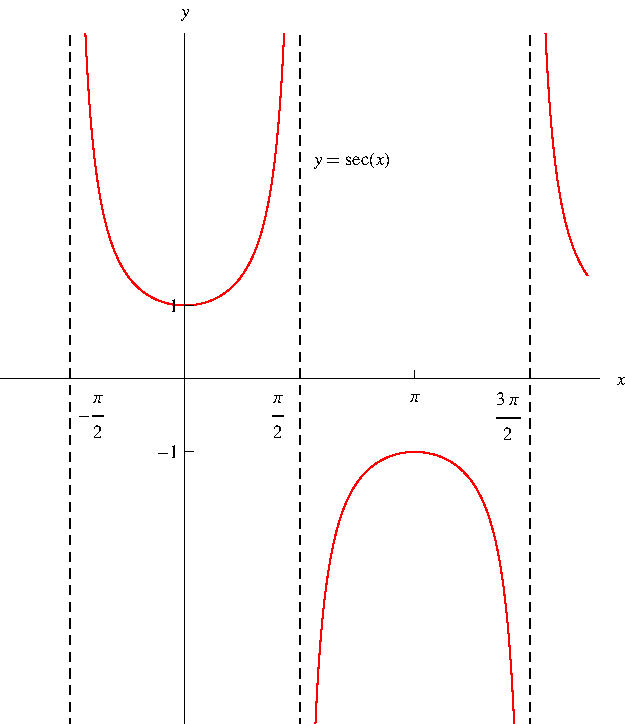
\includegraphics[width=5cm]{inverse-trig/pictures/07-06-seca.pdf}%
%}%
%\only<2->{%
%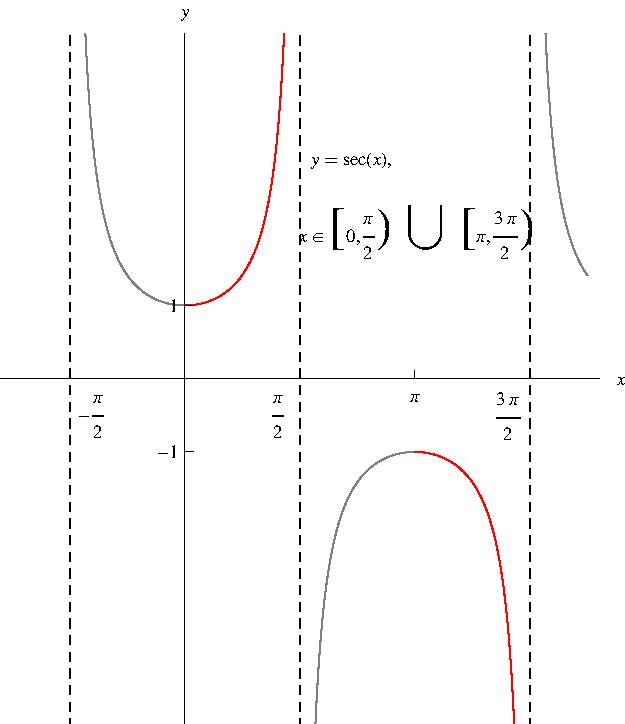
\includegraphics[width=5cm]{inverse-trig/pictures/07-06-secb.pdf}%
%}%
\column{0.57\textwidth}
\begin{itemize}
\item<2-> \noindent Plot $\sec x$.
\item<3-> Restrict domain to make one-to-one: Two common choices: \alertNoH{4}{$x\in \left[0, \frac{\pi}{2}\right)\cup\left(\frac{\pi}{2}, \pi \right] $} and \alertNoH{5}{$x\in \left[0, \frac{\pi}{2} \right) \cup \left[\pi,\frac{3\pi}{2} \right) $}.

\item<6-> $x\in \left[0, \frac{\pi}{2}\right)\cup\left(\frac{\pi}{2}, \pi \right] $ is good because the domain is easiest to remember: an interval without a point. \textbf{NOT our choice.}

\item<7,8,9,10-> $x\in \left[0, \frac{\pi}{2} \right) \cup \left[\pi,\frac{3\pi}{2} \right) $ is  good because $\tan x$ is positive on both intervals, resulting in easier differentiation and integration formulas. \textbf{Our choice.}

\end{itemize}
\end{columns}

\end{frame}